\section{Optimization}

\subsection{Restrictions}
As a reminder: $L$ is the length of the robot, and $w$ the width of the flywheel cylinders.
\begin{enumerate}
\item Not crashing with the ground at any inclination can be translated as:
\begin{figure}[ht]
	\centering
	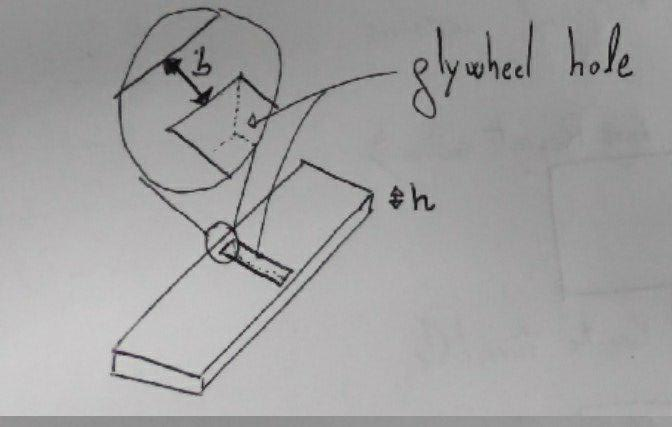
\includegraphics[width=5cm]{img/flywheel_hole.jpg}
	\caption{Flywheel hole diagram}
	\label{fig:Flywheel hole diagram}
\end{figure}
\[r_{wheel}> \sqrt{(r_{flywheel} + b)^2+(\frac{h}{2})^2}\]
\item We want to inserted the robot in to a external of diameter 0.5m so:
\begin{figure}[ht]
	\centering
	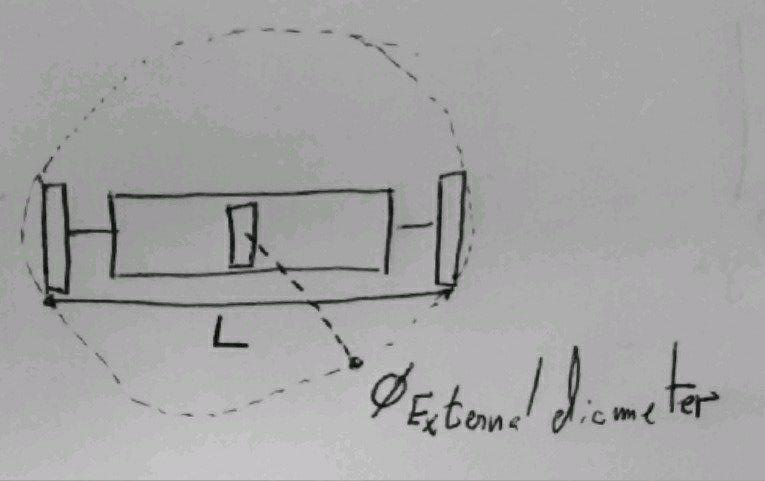
\includegraphics[width=5cm]{img/external_diameter.jpg}
	\caption{External diameter diagram}
	\label{fig:External diameter diagram}
\end{figure}
\[0.25 m > \sqrt{r_{wheel}^2 + L^2/4}\]
\item We can place all the devices:
\[L > 0.3m + w \]
\item Maximum weight of the robot: 5kg
\end{enumerate}

\subsection{Requirements}
\textbf{Flywheel mode}
\begin{enumerate}
	\item $\dot{y}_{max}$ (equation \ref{Maximum speed flywheel}) $> 0.1m/s$
	\item $\ddot{y}_{max}$ (equation \ref{maximum acceleration flywheel}) $0.01m/s^2$
	\item $h_{max}$ (equation \ref{Maximum height}) $> 0.001m$
	\item $sin(\alpha_{max})$ (equation \ref{Maximum angle using flywheel system}) $> 0.2$
\end{enumerate}
\textbf{pendulum mode}
\begin{enumerate}
	\item $\dot{y}_{max}$ (equation \ref{maximum speed pendulum}) $> 1m/s$
	\item $\ddot{y}_{max}$ (equation \ref{maximum acceleration pendulum}) $0.1m/s^2$
	\item $sin(\alpha_{max})$ (equation \ref{Maximum angle using pendulum system}) $> 0.02$
\end{enumerate}
	


\subsection{Cost function}
We will minimize the total mass.

\subsection{Results}
Our procedure has been making a grid with the three parameters of the robot design: $w$ (width of the cylinders), $r_{wheel}$ and $r_{flywheel}$.
We have fixed $r_{flywheel}$, iterated over the other two variables and keeped the best parameters for our cost function.

\begin{figure}[H]
	\centering
	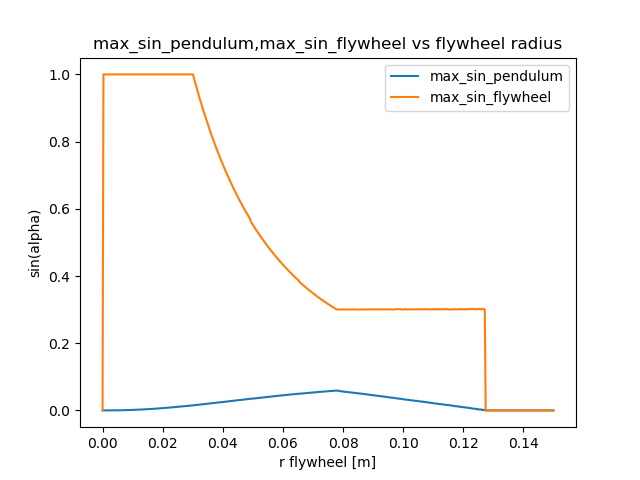
\includegraphics[width=10cm]{img/optimization/sin.png}
	\caption{Plot of the equations \ref{Maximum angle using flywheel system} and \ref{Maximum angle using pendulum system} at the parameters that maximize the cost function and fullfil the requirements and restrictions}
	\label{fig:Sinus plot}
\end{figure}
In figure \ref{fig:Sinus plot} we can see the evolution of our cost function (equation \ref{Maximum angle using pendulum system}) that has a maximum near $r_{flywheel} = 8cm$.
We can also check that we are fulfilling the requirements as long as $r_{flywheel}<13cm$ 

\begin{figure}[H]
	\centering
	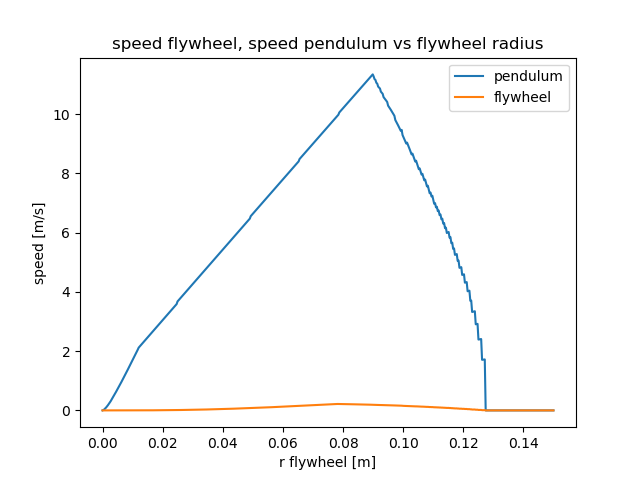
\includegraphics[width=10cm]{img/optimization/speed.png}
	\caption{Plot of the equations \ref{Maximum speed flywheel} and \ref{maximum speed pendulum} at the parameters that maximize the cost function and fullfil the requirements and restrictions}
	\label{fig:Speed plot}
\end{figure}
In figure \ref{fig:Speed plot} we can observe that the pendulum systems allows us to get a much higher speed than the flywheel.

\begin{figure}[H]
	\centering
	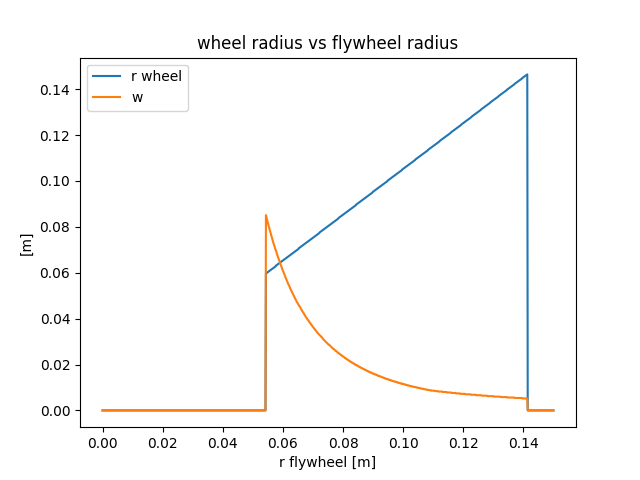
\includegraphics[width=10cm]{img/optimization/parameters.png}
	\caption{Plot of the parameters that maximize the cost function.}
	\label{fig:Parameters plot}
\end{figure}
Just for reference this plot in figure \ref{fig:Parameters plot} shows which parameters maximize the cost function so we can then design the robot accordingly.

\begin{figure}[H]
	\centering
	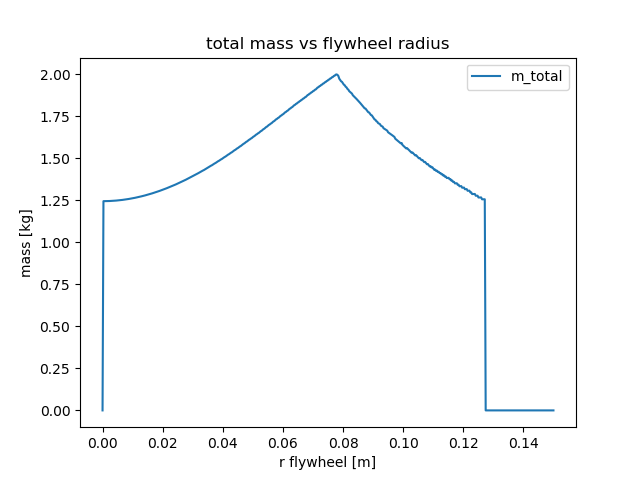
\includegraphics[width=10cm]{img/optimization/mass.png}
	\caption{Plot of the mass for each configuration.}
	\label{fig:Mass plot}
\end{figure}

Our selected parameters are:
\begin{center}
	\begin{tabular}{ |c|c|c| } 
	 \hline
	 $r_{flywheel}$ & $r_{wheel}$ & $w$ \\
	 \hline 
	 8cm & 9cm & 7cm \\ 
	 \hline
	\end{tabular}
	\end{center}

\subsection{Minimum section in the section of the flywheel}
\begin{figure}[ht]
	\centering
	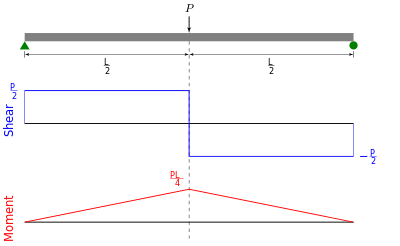
\includegraphics[width=10cm]{img/Shear_Moment_Diagram.png}
	\caption{Bendig moment diagram}
	\label{fig:Bendig moment diagram}
\end{figure}
The maximum bending moment is at the flywheel section:
\[M_y = \frac{P * L}{4}\]
Where P is the weight of the robot and L is the distance between the two wheels.

%The twisting moment $M_x$ in the body at the flywheel is the one we apply with the central motor.
%\[M_y = \tau_{motor}\]
%The pressure generated by this moment is:
%\[\tau=\frac{M_x}{\frac{1}{3}*}*R\]


\[I_y = \frac{2*b*h^3}{12}=\frac{b*h^3}{6}\]
\[\sigma=\frac{M_y}{I_y}*\frac{h}{2} = \frac{P*L}{48*b*h^2}\]
We are planning to build our body structure with aluminum:
\[\sigma_{al} = 400MPa = 4E8Pa\]
We will impose the relation:
\[b * 5 = h\]
And set a target P of $2000N$ and a maximum length of $0.5m$
\[\sigma_{al} = 4E8Pa = \frac{P*L}{48*b*h^2} = \frac{1000}{48*25*b^3} \]
Therefore:
\[b = \sqrt[3]{\frac{1000}{48*25*4E8}} = 0,001277182 m\]
We will use b=5mm and h=10mm from now on. Which is far more than what we need.

\subsection{Motor specifications}
Here we have the factory specifications of our motors: 
\begin{itemize}
    \item Operating voltage: between 3 V and 9 V
    \item Nominal voltage: 6 V
    \item Free-run speed at 6 V: 176 RPM
    \item Free-run current at 6 V: 80 mA
    \item Stall current at 6V: 900 mA
    \item Stall torque at 6V: 5 kg·cm
    \item Gear ratio: 1:35
    \item Reductor size: 21 mm
    \item Weight: 85 g
\end{itemize}
